\chapter{Future Plan \& Request for Feedback}\label{C:future}

\section{Future Stages}

The main components remaining for this project include the implementation, user study, evaluation, and the final report write-up. Currently we a SVD CF method working. Pending implementation sections include implementing neighbourhood CF methods. On the completion of these tasks, we must collect user information to test these methods. We are then able to run evaluation methods on real user data to obtain results. The main consideration is whether or not we want to test the performance or the prediction accuracy of the recommendation systems. Some feedback would be appreciated in terms of this.

\section{Evaluation Methods}

Since we are collecting like/dislike events from users, we would like a way to evaluate these methods. We would potentially like to evaluate these methods in terms of speed of recommendations, and prediction accuracy (depending on above). 

In terms of prediction accuracy, we are thinking of asking users to label food dishes. They will label the food dishes that they have tried before, labelling whether they liked the food dish, or whether they disliked the food dish. They will label as many of the food dishes as they can. We will then use 75\% of this data to train our model on, learning what they like. We will then use the remaining 25\% of the labelled data as a test set, using the recommender system to predict whether the user will like the remaining 25\% of the data. The prediction-accuracy will be based on how many recommendations that the system got right. 

In terms of performance, we are not sure on what to do to test this. 

\section{Other collaborative filtering methods}

Collaborative filtering has a range of different techniques. In the time frame given, it is difficult to test every method. In addition, parameters in collaborative filtering techniques also need to be tuned according to the data collected. In future, we plan to examine the neighbourhood CF techniques, comparing them with the SVD approach.

\section{Proposed Timeline}

We would like some feedback as to whether this project is feasible or not. Feedback regarding the evaluation plan would be kindly appreciated as well. 

\begin{figure}
\centering
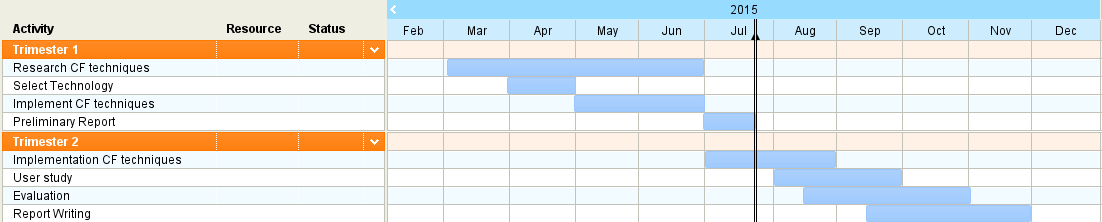
\includegraphics[scale=0.62]{gantt}
\caption{Full project Gantt Chart}
\label{fig:my_label}
\end{figure}

